\documentclass[11pt,a4j]{jarticle}
\usepackage{amsfonts}
\usepackage{amsmath}
\usepackage{authblk}
\usepackage{url} % URL
\usepackage{listings} % コードリスト
\usepackage[dvipdfmx]{graphicx}
\newcommand\norm[1]{\left\lVert#1\right\rVert}

% タイトル
\title{{KCF Trackerによる高速物体追跡}\thanks{慶應義塾大学 理工学研究科 2019春学期 "ComputerVision特論" 最終レポート} \\ }
% 著者名
\author{内海 佑麻\thanks{情報工学科4年,Email: uchiumi@ailab.ics.keio.ac.jp} (61602452)}
% 日付
\date{2019/07/25}

% 本文
\begin{document}
  % タイトル
  \maketitle
  % 要約
  \begin{abstract}
    モダンな物体追跡手法として,KCF Tracker (Kernelized Correlation Filter Tracker)を紹介し,実装をおこなった.
    KCF Trackerは,データ行列に巡回性を持たせることにより,DCTによる対角化が可能となり,処理にかかるストレージおよび計算量を大幅に削減することができる.
    さらに,カーネルトリックにより
  \end{abstract}
  % 目次
  \tableofcontents

  \newpage

  % 本文
  \section{はじめに}

    \subsection{Optical flow}
      異なる時点の2画像間で,各画素値の移動量を表現したベクトルをOptical Flowという.
      Optical Flowにより特徴点を検出することで,たとえば動画内の特定の物体を追跡することができる.
      まず,一般論として,勾配法(Gradient-based method)によるOptical Flowの求解手順を定式化する.
      勾配法では,Taylor展開による近似を用いるため,「連続する2画像での対象物の移動が微小であること」を前提としている.

      \paragraph{勾配法によるOptical Flowの求解}
      画像$I$における画素$(x,y)$の時刻$t$における画素値を$I(x,y,t)$,時間$\Delta t$に対する画素値の移動量を$(\Delta x, \Delta y)$とおく.
      移動前後で対象画素の画素値が不変であると仮定すると,

      \begin{align}
        I(x, ~ y, ~ t) = I(x + \Delta x, ~ y + \Delta y, ~ \Delta t)
      \end{align}

      が成り立つ.さらに,画素値の変化が滑らかであると仮定すると,1次までのTaylor展開により,以下の近似式を得る.

      \begin{align}
        I(x,y,t) \approx I(x,y,t) + \frac{\partial I}{\partial x} \Delta x + \frac{\partial I}{\partial y} \Delta y + \frac{\partial I}{\partial t} \Delta t
      \end{align}

      両辺を$\Delta t$で割って,整理すると,

      \begin{align}
        \frac{\partial I}{\partial x} \frac{\Delta x}{\Delta t} + \frac{\partial I}{\partial y} \frac{\Delta y}{\Delta t} + \frac{\partial I}{\partial t} = 0
      \end{align}

      $\Delta t \to 0$とすれば,

      \begin{align}
        \frac{\partial I}{\partial x} \frac{\partial x}{\partial t} + \frac{\partial I}{\partial y} \frac{\partial y}{\partial t} + \frac{\partial I}{\partial t} = 0
      \end{align}

      ここで,画素$(x,y)$のOptical Flow: $(u,v) = \left(\frac{\partial x}{\partial t}, \frac{\partial y}{\partial t} \right)$に着目する.
      $I_x = \frac{\partial I}{\partial x}$,$I_y = \frac{\partial I}{\partial y}$,$I_t = \frac{\partial I}{\partial t}$,とおけば,
      $(u,v)$がみたすべき方程式\footnote{これを,OpticalFlowの拘束式と呼ぶ.}は,次式のようになる.

      \begin{align}
        I_x u + I_y v + I_t = 0
      \end{align}

      しかし,上式は2つの未知数$u,v$に対して方程式は1つであり,解が定まらない\footnote{これを,Aperture Problem(窓問題)という.}.\cite{Szeliski:2010:CVA:1941882}
      そのため,上式に加えて,いくつかの仮定(制約条件)を導入してOptical Flow: $(u,v)$を球解する手法が提案されている.
      古典的で重要な手法として,Lucas–Kanade法やHorn–Schunck法がある.\cite{Horn:1980:DOF:888857}\cite{Lucas:1981:IIR:1623264.1623280}\cite{Harris88acombined}\cite{Tomasi91detectionand}

      \begin{itemize}
        \item Lucas–Kanade法 \\
          「各画素の近傍では,移動方向が相関する」という仮定をおく.
          画像中の特定の点(領域)に絞って追跡を行うような用途に適しているため,sparse型と呼ばれる.
        \item Horn–Schunck法 \\
          「各画素は,変化率が最小となる方向へ移動する」という仮定をおく.
          画像中の画素全体の動きを解析するような用途に適しているため,dense型と呼ばれる.
      \end{itemize}      

  \section{理論}
    Kernelized Correlation Filters\cite{DBLP:journals/corr/HenriquesCMB14}について解説する.

    \subsection{Ridge回帰}
      SVMなどの洗練されたモデルに近い性能をもち,かつ単純な閉形式解\footnote{四則演算と初等関数の合成関数によって表せる解を,閉形式解(closed-form solution)という.}をもつRidge回帰を用いる.
      $n$個の訓練データ${({\bf x}_i, y_i)}_{i = 1 \cdots n}$に対するRidge回帰は,以下のように定式化される.
      \begin{align}
        \min_{\bf w} \sum_{i=1}^{n} { \left( f({\bf x}_i) - y_i \right) }^{2} + \lambda {\norm{ \bf w }}^{2}, ~~~
        f({\bf x}_i) = {\bf w}^{\mathrm{T}} {\bf x}_i
      \end{align}
      データ行列
      \begin{align}
        X = 
        \left[
          \begin{array}{c}
            x_{1}^{\mathrm{T}} \\
            x_{2}^{\mathrm{T}} \\
            x_{3^{\mathrm{T}}} \\
            \vdots \\
            x_{N}^{\mathrm{T}} 
          \end{array}
        \right]
        =
        \left[
          \begin{array}{ccccc}
            x_{11} & x_{12} & x_{13} & \cdots & x_{1n} \\
            x_{21} & x_{22} & x_{23} & \cdots & x_{2n} \\
            x_{31} & x_{32} & x_{33} & \cdots & x_{3n} \\
            \vdots&\vdots&\ddots&\ddots&\vdots \\
            x_{n1} & x_{n2} & x_{n3} & \cdots & x_{nn} 
          \end{array}
        \right]
      \end{align}
      を用いると,Ridge回帰の閉形式解は,以下のようになる.
      \begin{align}
        {\bf w} = { ({X}^{\mathrm{T}} X + \lambda I) }^{-1} {X}^{\mathrm{T}} {\bf y}
      \end{align}
      さらに,転置行列$X^{\mathrm{T}}$を,エルミート転置$X^{\mathrm{H}} := {(X^{*})}^{\mathrm{T}}$によって拡張すると,
      \begin{align}
        {\bf w} = { ({X}^{\mathrm{H}} X + \lambda I) }^{-1} {X}^{\mathrm{H}} {\bf y}
      \end{align}
      となる.\footnote{$A^{*}$は,行列$A$の複素共役を表す.}

    \subsection{巡回行列とDFT}
      注目点の移動パスをベクトル${\bf x} = {(x_1, \cdots x_n)}^{\mathrm{T}} \in \mathbb{R}^{n}$とおく.このとき,cyclic shift operatorとして,$n \times n$行列
      \begin{align}
        P = 
        \left[
          \begin{array}{ccccc}
            0 & 0 & 0 & \cdots & 1 \\
            1 & 0 & 0 & \cdots & 0 \\
            0 & 1 & 0 & \cdots & 0 \\
            \vdots&\vdots&\ddots&\ddots&\vdots \\
            0 & 0 & \cdots & 1 & 1
          \end{array}
        \right]
      \end{align}
      を定義すると,ベクトル${\bf x}$の巡回置換は,
      \begin{align}
        \left\{ {P}^{u}{\bf x} ~|~ u=0,\cdots n-1 \right\}
      \end{align}
      と得られる.すなわち,あるベクトル$\bf x$から,$n$個の仮想サンプルを作成することができる.
      そこで,ある信号$\bf x$を,$P$を用いて拡張すると,
      \begin{align}
        C({\bf x}) = 
        \left[
          \begin{array}{c}
            {({P}^{0} {\bf x})}^{\mathrm{T}} \\
            {({P}^{1} {\bf x})}^{\mathrm{T}} \\
            {({P}^{2} {\bf x})}^{\mathrm{T}} \\
            \vdots \\
            {({P}^{n-1} {\bf x})}^{\mathrm{T}} 
          \end{array}
        \right]
        = 
        \left[
          \begin{array}{ccccc}
            x_1 & x_2 & x_3 & \cdots & x_n \\
            x_n & x_1 & x_2 & \cdots & x_{n-1} \\
            x_{n-1} & x_n & x_1 & \cdots & x_{n-2} \\
            \vdots&\vdots&\vdots&\ddots&\vdots \\
            x_2 & x_3 & x_4 & \cdots  & x_1
          \end{array}
        \right]
      \end{align}
      を得られる.ここで,$C({\bf x})$は巡回行列(Circulant matrix)だから,これはDFT(Discrete Fourier Transform)によって対角化可能である.
      すなわち,
      \begin{align}
        \forall {\bf z} \in \mathbb{R}^{n}, ~~ F({\bf z}) = \sqrt{n} F{\bf z}
      \end{align}
      をみたす,ある定まったDFT行列$F$と,$\bf x$の周波数成分
      \begin{align}
        \hat{\bf x} = F({\bf x}) = \sqrt{n} F{\bf x}
      \end{align}
      を用いると,$C({\bf x})$は次式のように固有値分解できる.
      \begin{align}
        C({\bf x}) = F {\rm diag} (\hat{\bf x}) {F}^{H}
      \end{align}

    \subsection{巡回行列を使ったRidge回帰}
      $C({\bf x})$をデータ行列として,Ridge回帰を行う,中心化していない共分散行列は,DCT行列$F$を用いて次式のように表せる.
      \begin{align}
        {C({\bf x})}^{\mathrm{H}}C({\bf x}) = F {\rm diag} (\hat{{\bf x}}^{*}) {F}^{H} F {\rm diag} (\hat{\bf x}) {F}^{H}
      \end{align}
      さらに,要素積$\odot$を用いて
      \begin{align}
        F^{H}F = {( F^{*} )}^{\mathrm{T}} F &= I \\
        {\rm diag} (\hat{{\bf x}}^{*})\cdot {\rm diag} (\hat{\bf x}) &= {\rm diag} ( \hat{{\bf x}}^{*} \odot \hat{\bf x} )
      \end{align}
      が成り立つから,
      \begin{align}
        {C({\bf x})}^{\mathrm{H}}C({\bf x}) = F {\rm diag} ( \hat{{\bf x}}^{*} \odot \hat{\bf x} ) {F}^{H}
      \end{align}
      となる.
      ここで,$\hat{{\bf x}}^{*} \odot \hat{\bf x}$は,信号$\bf x$の自己相関(auto correlation)またはパワースペクトル(power spectrum)と呼ばれる量である.
      すなわち,$P$によって空間方向にシフトさせた信号どうしの共分散を表している.
      以上から,データ行列として$C({\bf x})$を用いたRidge回帰の閉形式解は,次のようになる.
      \begin{align}
        \hat{\bf w} &= { ({C({\bf x})}^{\mathrm{H}} C({\bf x}) + \lambda I) }^{-1} {C({\bf x})}^{\mathrm{H}} \hat{\bf y} \\
                &= {\rm diag} \left( \frac{{\hat{\bf x}}^{*}}{\hat{{\bf x}}^{*} \odot \hat{\bf x} + \lambda} \right) \hat{\bf y} \\
                &= \frac{{\hat{\bf x}}^{*} \odot \hat{\bf y}}{\hat{{\bf x}}^{*} \odot \hat{\bf x} + \lambda} \\
      \end{align}
      よって,逆DFT${F}^{-1}$を用いて,$w$が求められる.
      \begin{align}
        {\bf w} = {F}^{-1}( \hat{\bf w} )
      \end{align}

    \subsection{Kernel Ridge回帰}
      任意の正定値関数$k({\bf x}_i, {\bf x}_j) = {\phi({\bf x}_i)}^{\mathrm{T}} \phi({\bf x}_j)$に対して,
      \begin{align}
        {\bf w} = \sum_{i=1}^{n} \alpha_i \phi({\bf x}_i)
      \end{align}
      とおけば,グラム行列
      \begin{align}
        K = 
        \left[
          \begin{array}{ccccc}
            k({\bf x}_1, {\bf x}_1) & k({\bf x}_1, {\bf x}_2) & k({\bf x}_1, {\bf x}_3) & \cdots & k({\bf x}_1, {\bf x}_n) \\
            k({\bf x}_2, {\bf x}_1) & k({\bf x}_2, {\bf x}_2) & k({\bf x}_2, {\bf x}_3) & \cdots & k({\bf x}_2, {\bf x}_n) \\
            k({\bf x}_3, {\bf x}_1) & k({\bf x}_3, {\bf x}_2) & k({\bf x}_3, {\bf x}_3) & \cdots & k({\bf x}_3, {\bf x}_n) \\
            \vdots&\vdots&\ddots&\ddots&\vdots \\
            k({\bf x}_n, {\bf x}_1) & k({\bf x}_n, {\bf x}_2) & k({\bf x}_n, {\bf x}_3) & \cdots & k({\bf x}_n, {\bf x}_n)
          \end{array}
        \right]
      \end{align}
      を用いて,Representer定理より,
      \begin{align}
        f({\bf x}_i) = {\bf w}^{\mathrm{T}} {\bf x}_i &= \sum_{j=1}^{n} \alpha_j k({\bf x}_i, {\bf x}_j) \\
        {\norm{ \bf w }}^{2} &= {\bf \alpha}^{\mathrm{T}} K {\bf \alpha}
      \end{align}
      が成り立つ.
      すなわち,$n$個の訓練データ${({\bf x}_i, y_i)}_{i = 1 \cdots n}$に対するKernel Ridge回帰は,以下のように定式化される.
      \begin{align}
        \min_{\bf \alpha} \sum_{i=1}^{n} { \left( f({\bf x}_i) - y_i \right) }^{2} + \lambda {\bf \alpha}^{\mathrm{T}} K {\bf \alpha}, ~~~
        f({\bf x}_i) =  \sum_{j=1}^{n} \alpha_j k({\bf x}_i, {\bf x}_j)
      \end{align}
      Kernel Ridge回帰の閉形式解は,以下のようになる.
      \begin{align}
        {\bf \alpha} = { ( K + \lambda I ) }^{-1} {\bf y}
      \end{align}

    \subsection{巡回行列を使ったKernel Ridge回帰}
      Ridge回帰と同様に,ベクトル${\bf x}$とその巡回シフトに対するカーネルは,$P$と$k(\cdot,\cdot)$を用いて
      \begin{align}
        \left\{ k({\bf x}, {P}^{u}{\bf x}) ~|~ u=0,\cdots n-1 \right\} 
      \end{align}
      となる.よって,ベクトル${\bf {k}^{xx}}$を,
      \begin{align}
        {\bf k^{xx}_{i}} = k({\bf x}, {P}^{i-1}{\bf x}) ~~~ (i=1,\cdots n)
      \end{align}
      と定義し,これを用いた巡回行列
      \begin{align}
        C({\bf k^{xx}}) = 
        \left[
          \begin{array}{c}
            {({P}^{0} {\bf k^{xx}})}^{\mathrm{T}} \\
            {({P}^{1} {\bf k^{xx}})}^{\mathrm{T}} \\
            \vdots \\
            {({P}^{n-1} {\bf k^{xx}})}^{\mathrm{T}} 
          \end{array}
        \right]
        = 
        \left[
          \begin{array}{cccc}
            k({\bf x}, P^{0}{\bf x}) & k({\bf x}, P^{1}{\bf x}) & \cdots & k({\bf x}, P^{n-1}{\bf x}) \\
            k({\bf x}, P^{n-1}{\bf x}) & k({\bf x}, P^{0}{\bf x}) & \cdots & k({\bf x}, P^{n-2}{\bf x}) \\
            \vdots&\vdots&\ddots&\vdots \\
            k({\bf x}, P^{1}{\bf x}) & k({\bf x}, P^{2}{\bf x}) &  \cdots & k({\bf x}, P^{0}{\bf x}) 
          \end{array}
        \right]
      \end{align}

      を得られる.さらに,中心化していない共分散行列は,DCT行列$F$を用いて次式のように表せる.

      \begin{align}
        {C( {\bf {k}^{xx}} ) }^{\mathrm{H}} C( {\bf {k}^{xx}} ) = F {\rm diag} \left( {\bf {\hat{k^*}}^{xx}} \odot {\bf {\hat{k}}^{xx} } \right) {F}^{\mathrm{H}} 
      \end{align}

      以上から,データ行列として$C({\bf {k}^{xx}})$を用いたKernel Ridge回帰の閉形式解は,次のようになる.

      \begin{align}
        \hat{\bf \alpha} &= { ( C( {\bf {k}^{xx}} ) + \lambda I ) }^{-1} {\bf y} \\
                &= \frac{\hat{\bf y}}{ {\bf {\hat{k}}^{xx} } + \lambda }
      \end{align}

      よって,逆DFT${F}^{-1}$を用いて,$w$が求められる.

      \begin{align}
        {\bf \alpha} = {F}^{-1}( \hat{\bf \alpha} )
      \end{align}
  
      
  \section{実装}

    RBF kernelを用いる.

    \begin{align}
      {\bf {k}^{xx'}} = \exp \left\{ - \frac{1}{\sigma^2} \left( \norm{\bf x}^{2} + \norm{\bf x'}^{2} - 2 {F}^{-1} ( \hat{{\bf x}}^{*} \odot \hat{\bf x}' ) \right) \right\}
    \end{align}

    \paragraph{実行環境}
    以下の環境でプログラムを実装した.主要なスクリプトの記述にはPythonを採用した.
    使用したコードは,\url{https://github.com/yumaloop/CV_report2019}で公開した.

    \begin{itemize}
      \item OS: macOS Mojave 10.14.4
      \item App: QuickTime Player 10.5 (935.3), iMovie (10.1.12)
      \item Lang: Python 3.7.4
      \item Lib: Numpy 1.16.1, Opencv-python 4.1.0
    \end{itemize}

    なお,今回は,KCF Trackerアルゴリズムのみを実装したため,動画の入出力やユーザインターフェースは,OpenCVの定義済み関数を利用した.
    具体的に,KCF Trackerのオブジェクトをインポートできる$\rm OpenCVのcv2.TrackerKCF\_create()$を使って,Object Trackingを行うコードは次のようになる.
    このうち,コード中のオブジェクト$\rm tracker$と関連する処理を実装した.
    
    \begin{lstlisting}[basicstyle=\ttfamily\footnotesize, frame=single]
      import sys
      import cv2

      # Set up tracker as KCF.
      tracker = cv2.TrackerKCF_create()

      # cap: captured images from the video
      input_file = "********.mp4"
      cap = cv2.VideoCapture(input_file)
      cap_width  = int(cap.get(cv2.CAP_PROP_FRAME_WIDTH))
      cap_height = int(cap.get(cv2.CAP_PROP_FRAME_HEIGHT))
      cap_size = (cap_width, cap_height)
  
      # out: result video (m4v)
      # see also https://gist.github.com/takuma7/44f9ecb028ff00e2132e
      output_file = "********.m4v"
      fourcc = cv2.VideoWriter_fourcc('m', 'p', '4', 'v')  
      out = cv2.VideoWriter(output_file, fourcc, 20.0, cap_size)
    
      # Exit if video not opened.
      if not cap.isOpened():
          print("Cannot open the video file.")
          sys.exit()
    
      # Read first frame.
      ret, frame = cap.read()
      if not ret:
          print('Cannot read the video file.')
          sys.exit()
        
      # Initialize bounding box
      bbox = (287, 23, 86, 320)
      # Uncomment the line below to select a different bounding box
      bbox = cv2.selectROI(frame, False)
    
      # Initialize tracker
      ret = tracker.init(frame, bbox)

      while True:
      # Read a new frame
      ret, frame = cap.read()
      if not ret: break

      # =================================================
      ''' Update tracker (Tracking process in OpenCV) '''
      ret, bbox = tracker.update(frame) 
      # =================================================

      # Draw bounding box
      if ret:
          # Tracking succeeded
          p1 = (int(bbox[0]), int(bbox[1]))
          p2 = (int(bbox[0] + bbox[2]), int(bbox[1] + bbox[3]))
          cv2.rectangle(frame, p1, p2, (255,0,0), 2, 1)
      else :
          # Tracking failed
          cv2.putText(frame, "Tracking failure detected", 
          (100, 80), cv2.FONT_HERSHEY_SIMPLEX, 0.75, (0,0,255) ,2)

      # Display result
      cv2.imshow("Tracking", frame)

      # Save result as mp4 file
      out.write(frame)

      # Exit if ESC pressed
      k = cv2.waitKey(1) & 0xff
      if k == 27:
          break
    \end{lstlisting}

    \paragraph{出力結果}
    まず.chaplin.mp4で

    % fig1 chaplin opencv
    \begin{figure}[hbtp]
      \begin{center}
        \includegraphics[clip,width=12.5cm]{./figures/chaplin_kcf_opencv.jpg}
        \caption{chaplin.mp4に対して,OpenCV KCF Trackerで物体追跡を行なった結果}
        \label{fig:AC_PetriNet}
      \end{center}
    \end{figure}

    % fig2 chaplin impl
    \begin{figure}[hbtp]
      \begin{center}
        \includegraphics[clip,width=12.5cm]{./figures/chaplin_kcf_impl.jpg}
        \caption{chaplin.mp4に対して,実装した KCF Trackerで物体追跡を行なった結果}
        \label{fig:AC_PetriNet}
      \end{center}
    \end{figure}

    % fig3 car1 opencv
    \begin{figure}[hbtp]
      \begin{center}
        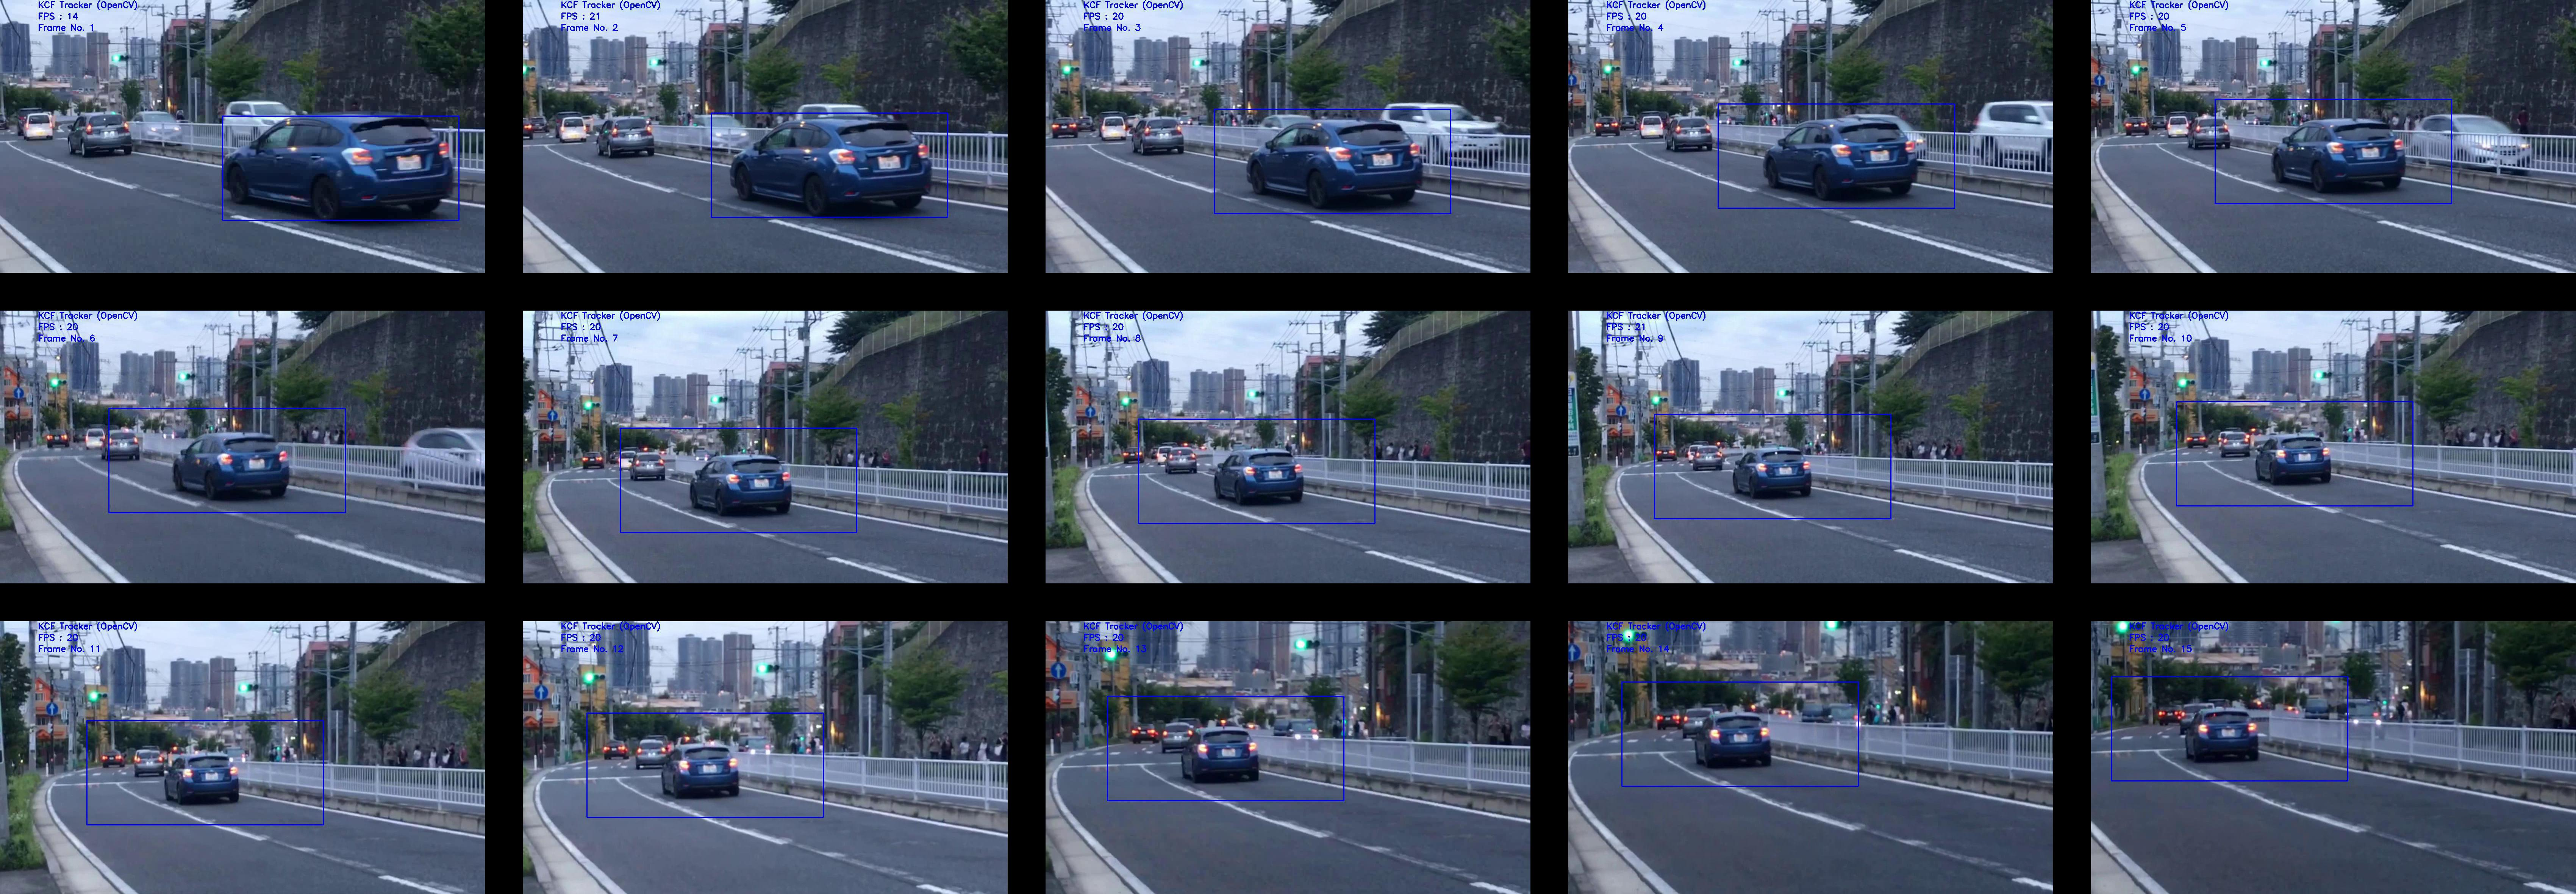
\includegraphics[clip,width=12.5cm]{./figures/car1_kcf_opencv.jpg}
        \caption{car1.mp4に対して,OpenCV KCF Trackerで物体追跡を行なった結果}
        \label{fig:AC_PetriNet}
      \end{center}
    \end{figure}

    % fig4 car1 impl
    \begin{figure}[hbtp]
      \begin{center}
        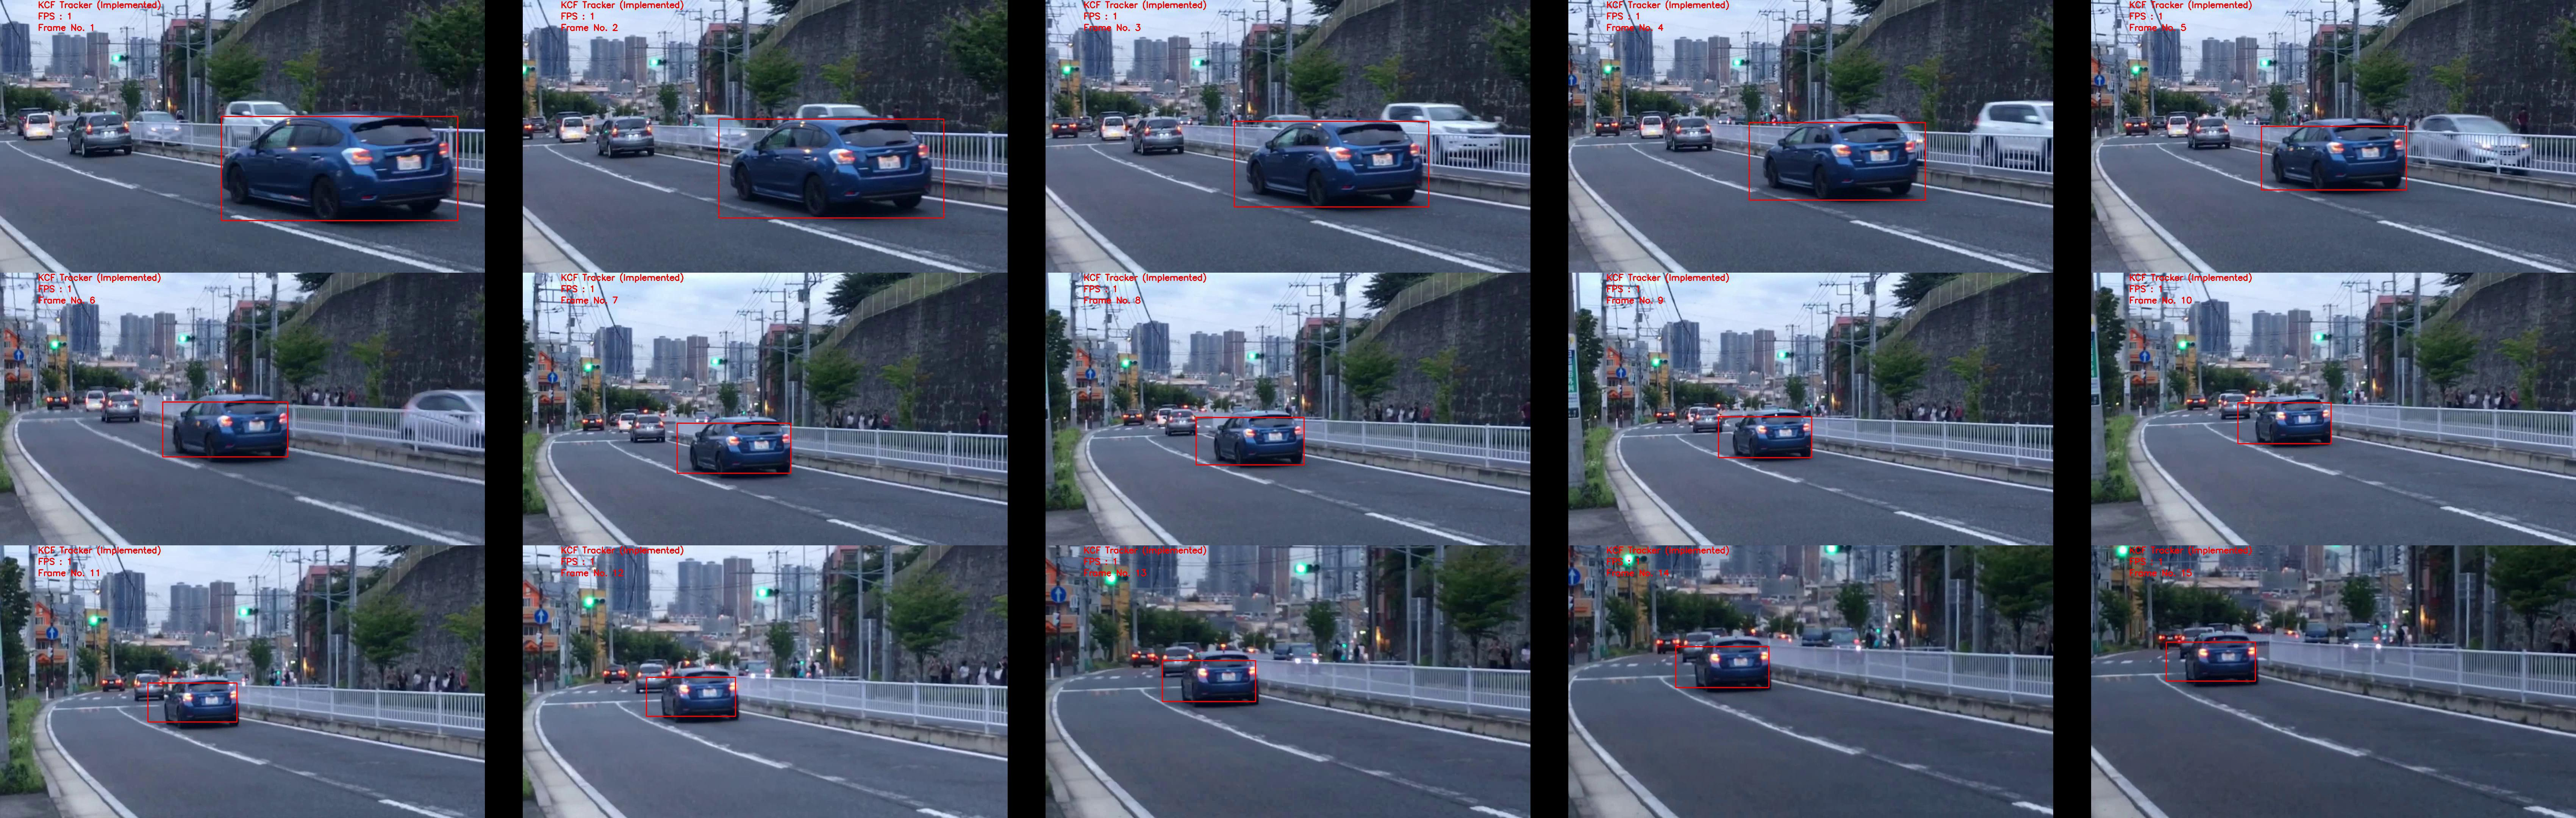
\includegraphics[clip,width=12.5cm]{./figures/car1_kcf_impl.jpg}
        \caption{car1.mp4に対して,実装した KCF Trackerで物体追跡を行なった結果}
        \label{fig:AC_PetriNet}
      \end{center}
    \end{figure}

    % fig5 car2 opencv
    \begin{figure}[hbtp]
      \begin{center}
        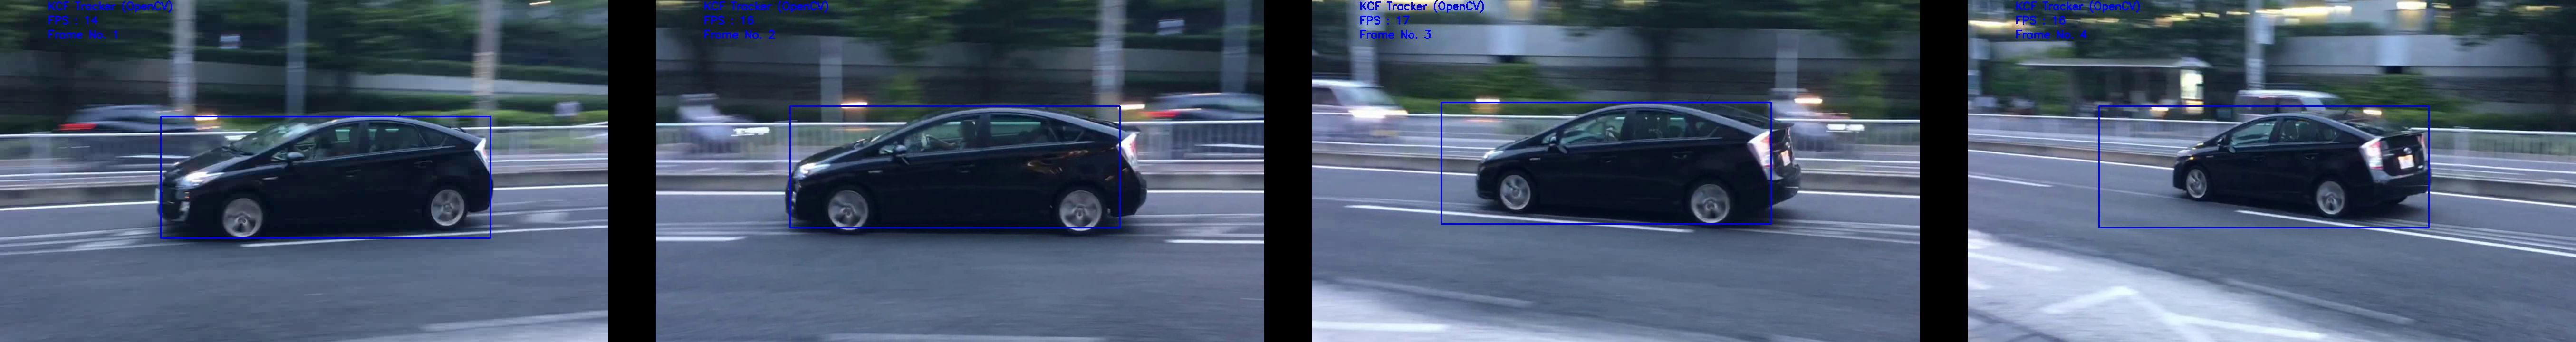
\includegraphics[clip,width=12.5cm]{./figures/car2_kcf_opencv.jpg}
        \caption{car2.mp4に対して,OpenCV KCF Trackerで物体追跡を行なった結果}
        \label{fig:AC_PetriNet}
      \end{center}
    \end{figure}

    % fig6 car2 impl
    \begin{figure}[hbtp]
      \begin{center}
        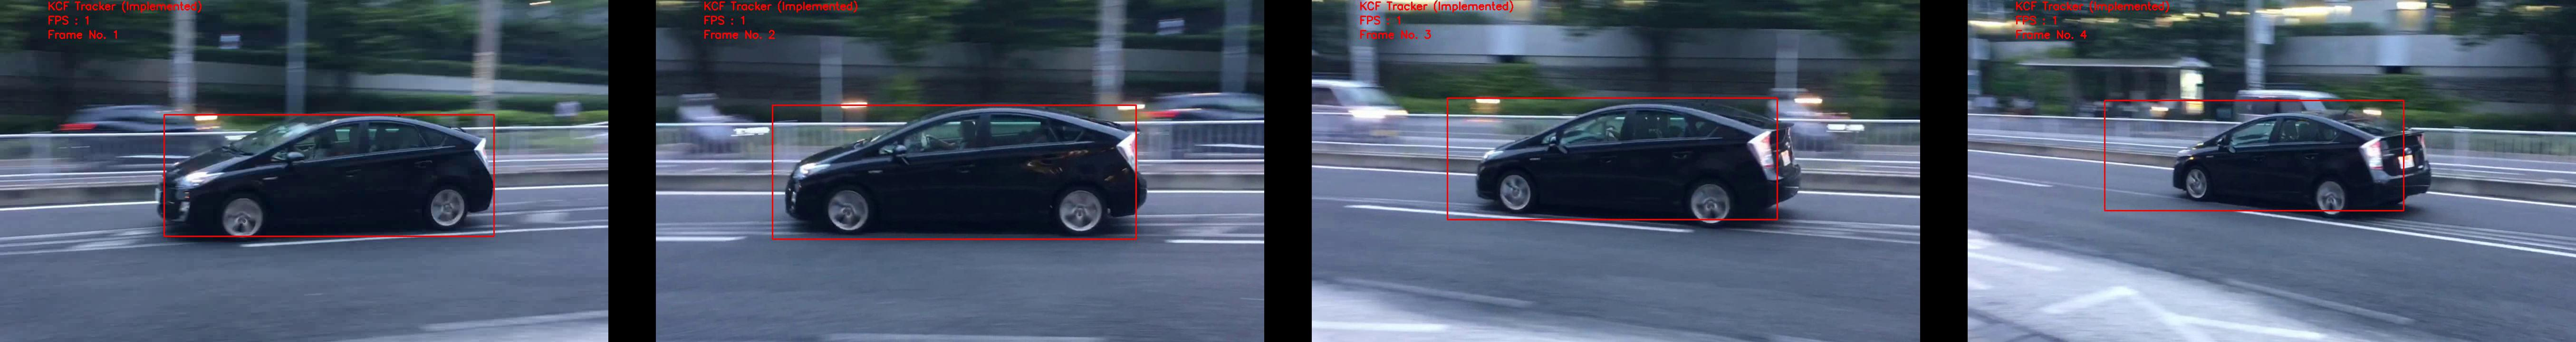
\includegraphics[clip,width=12.5cm]{./figures/car2_kcf_impl.jpg}
        \caption{car2.mp4に対して,実装した KCF Trackerで物体追跡を行なった結果}
        \label{fig:AC_PetriNet}
      \end{center}
    \end{figure}

    % fig7 bus1 opencv
    \begin{figure}[hbtp]
      \begin{center}
        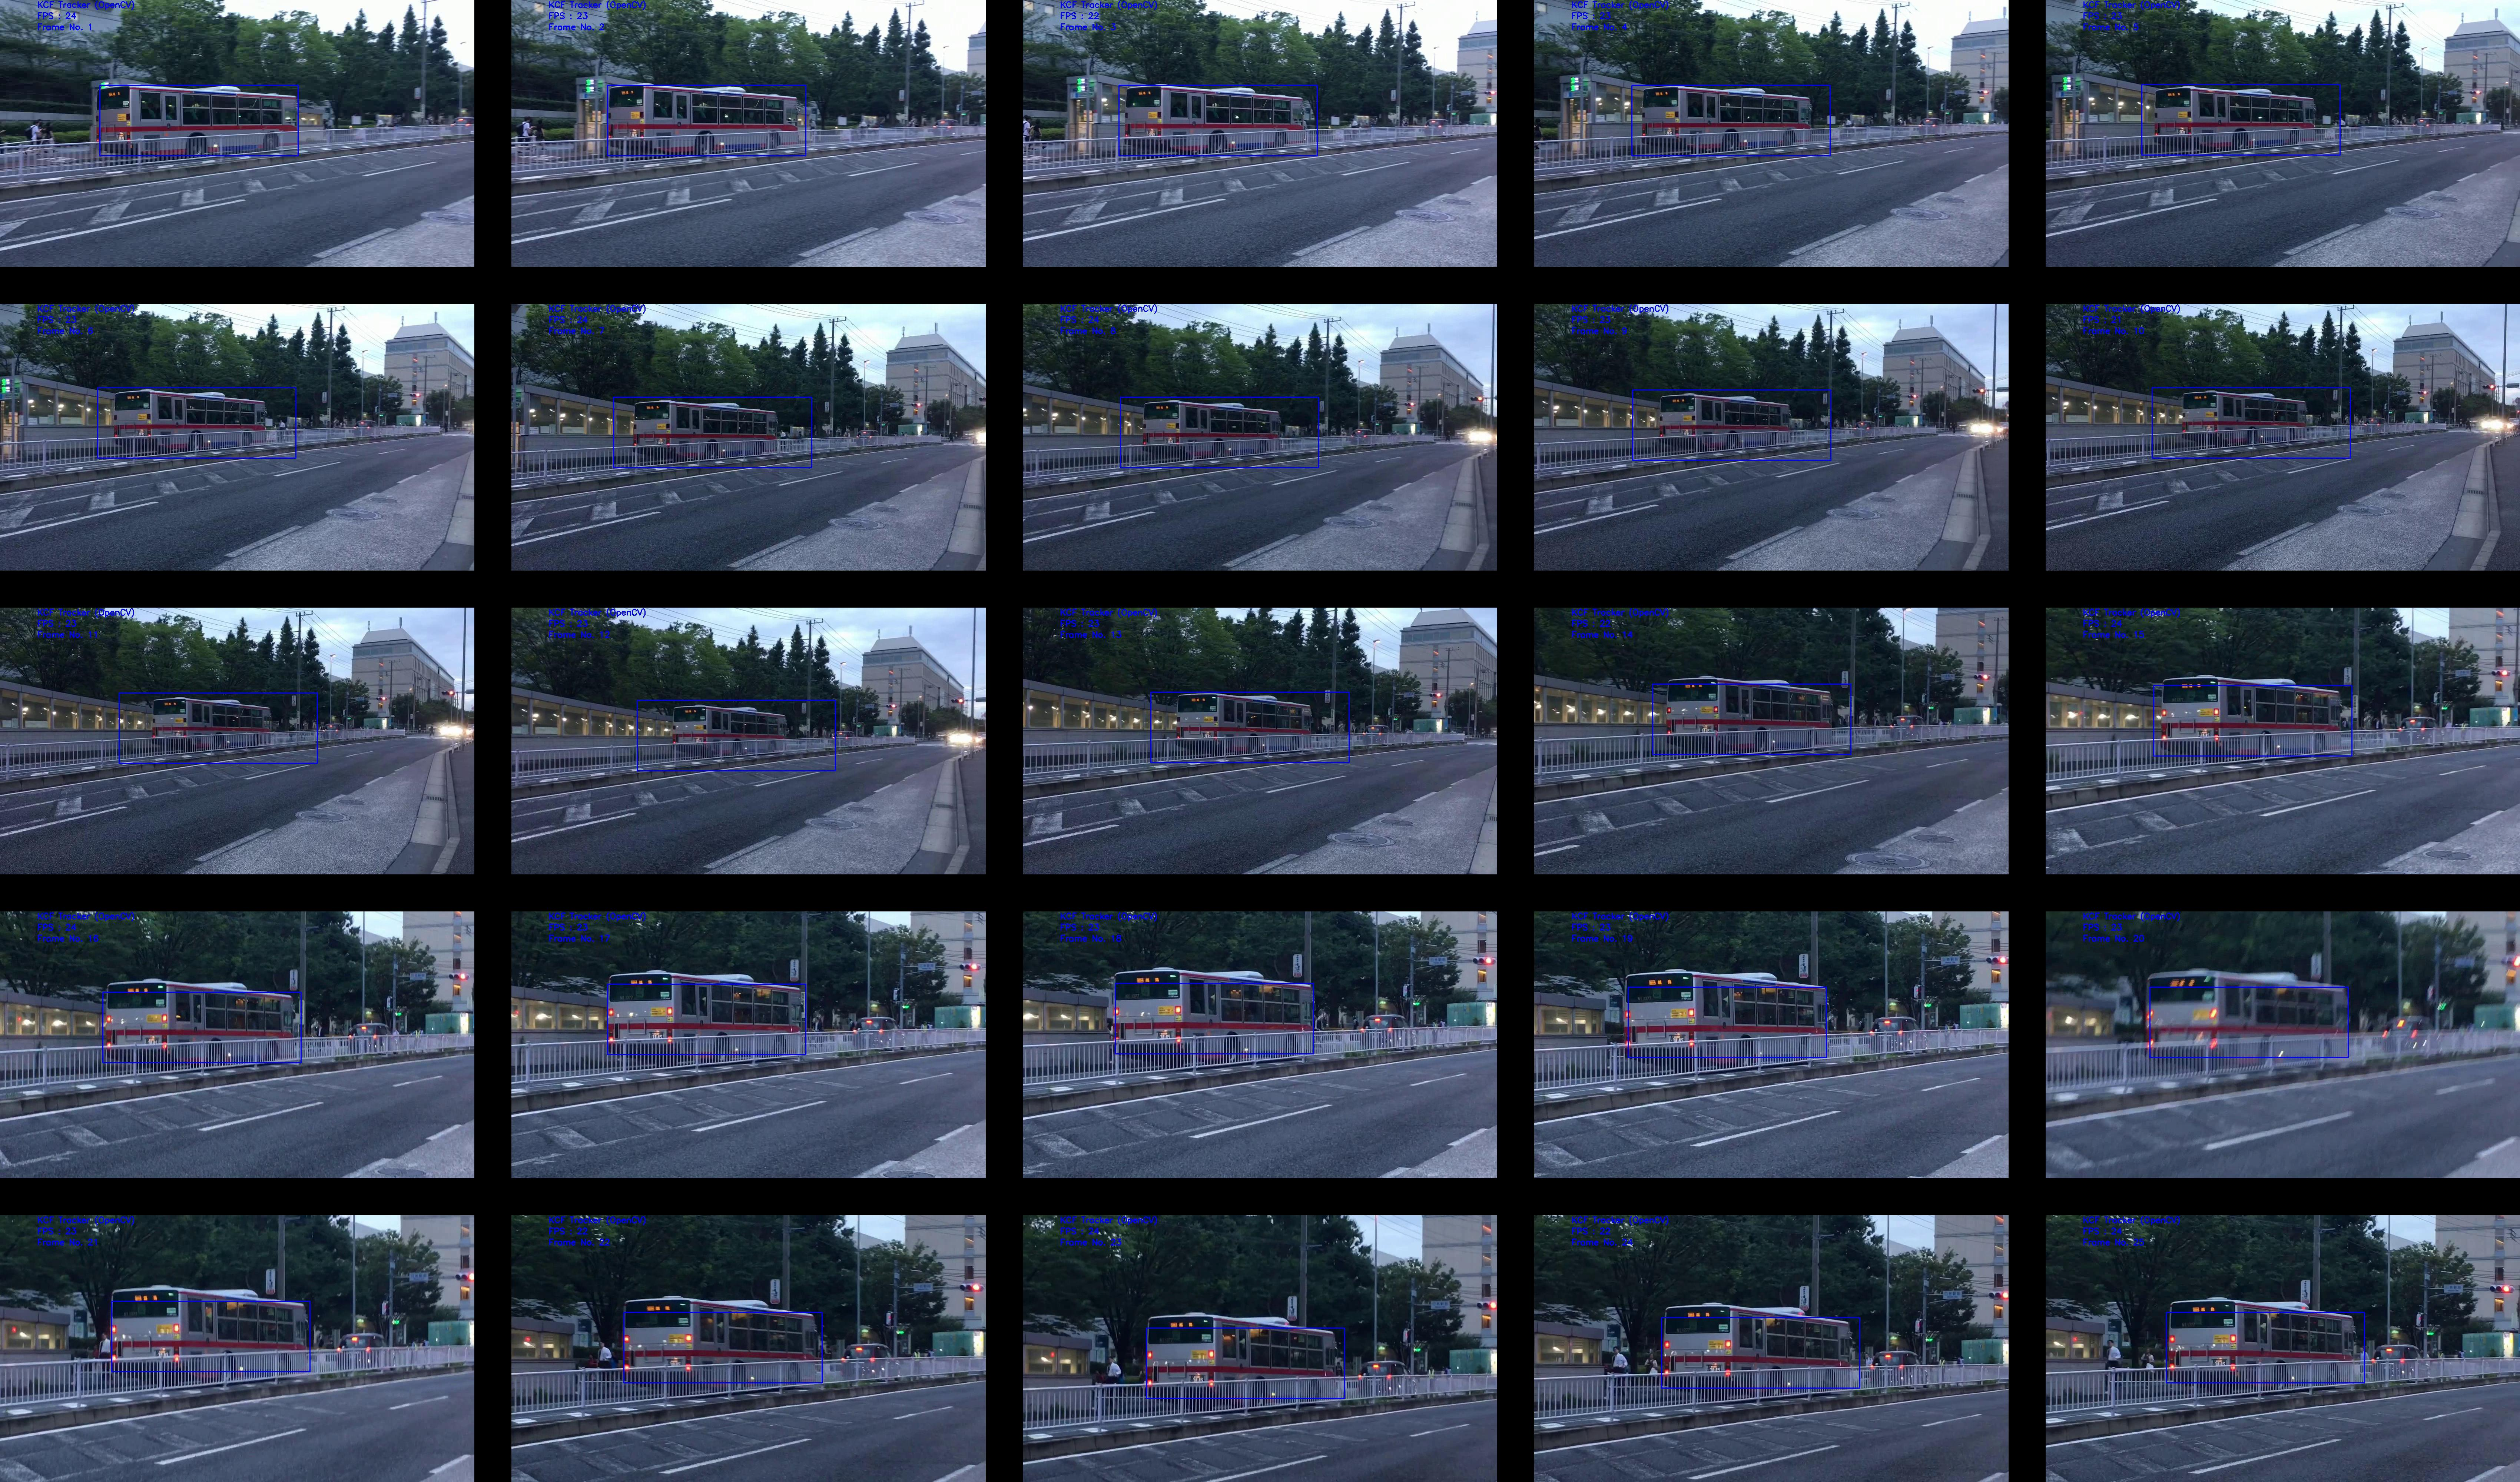
\includegraphics[clip,width=12.5cm]{./figures/bus1_kcf_opencv.jpg}
        \caption{bus1.mp4に対して,OpenCV KCF Trackerで物体追跡を行なった結果}
        \label{fig:AC_PetriNet}
      \end{center}
    \end{figure}

    % fig8 bus1 impl
    \begin{figure}[hbtp]
      \begin{center}
        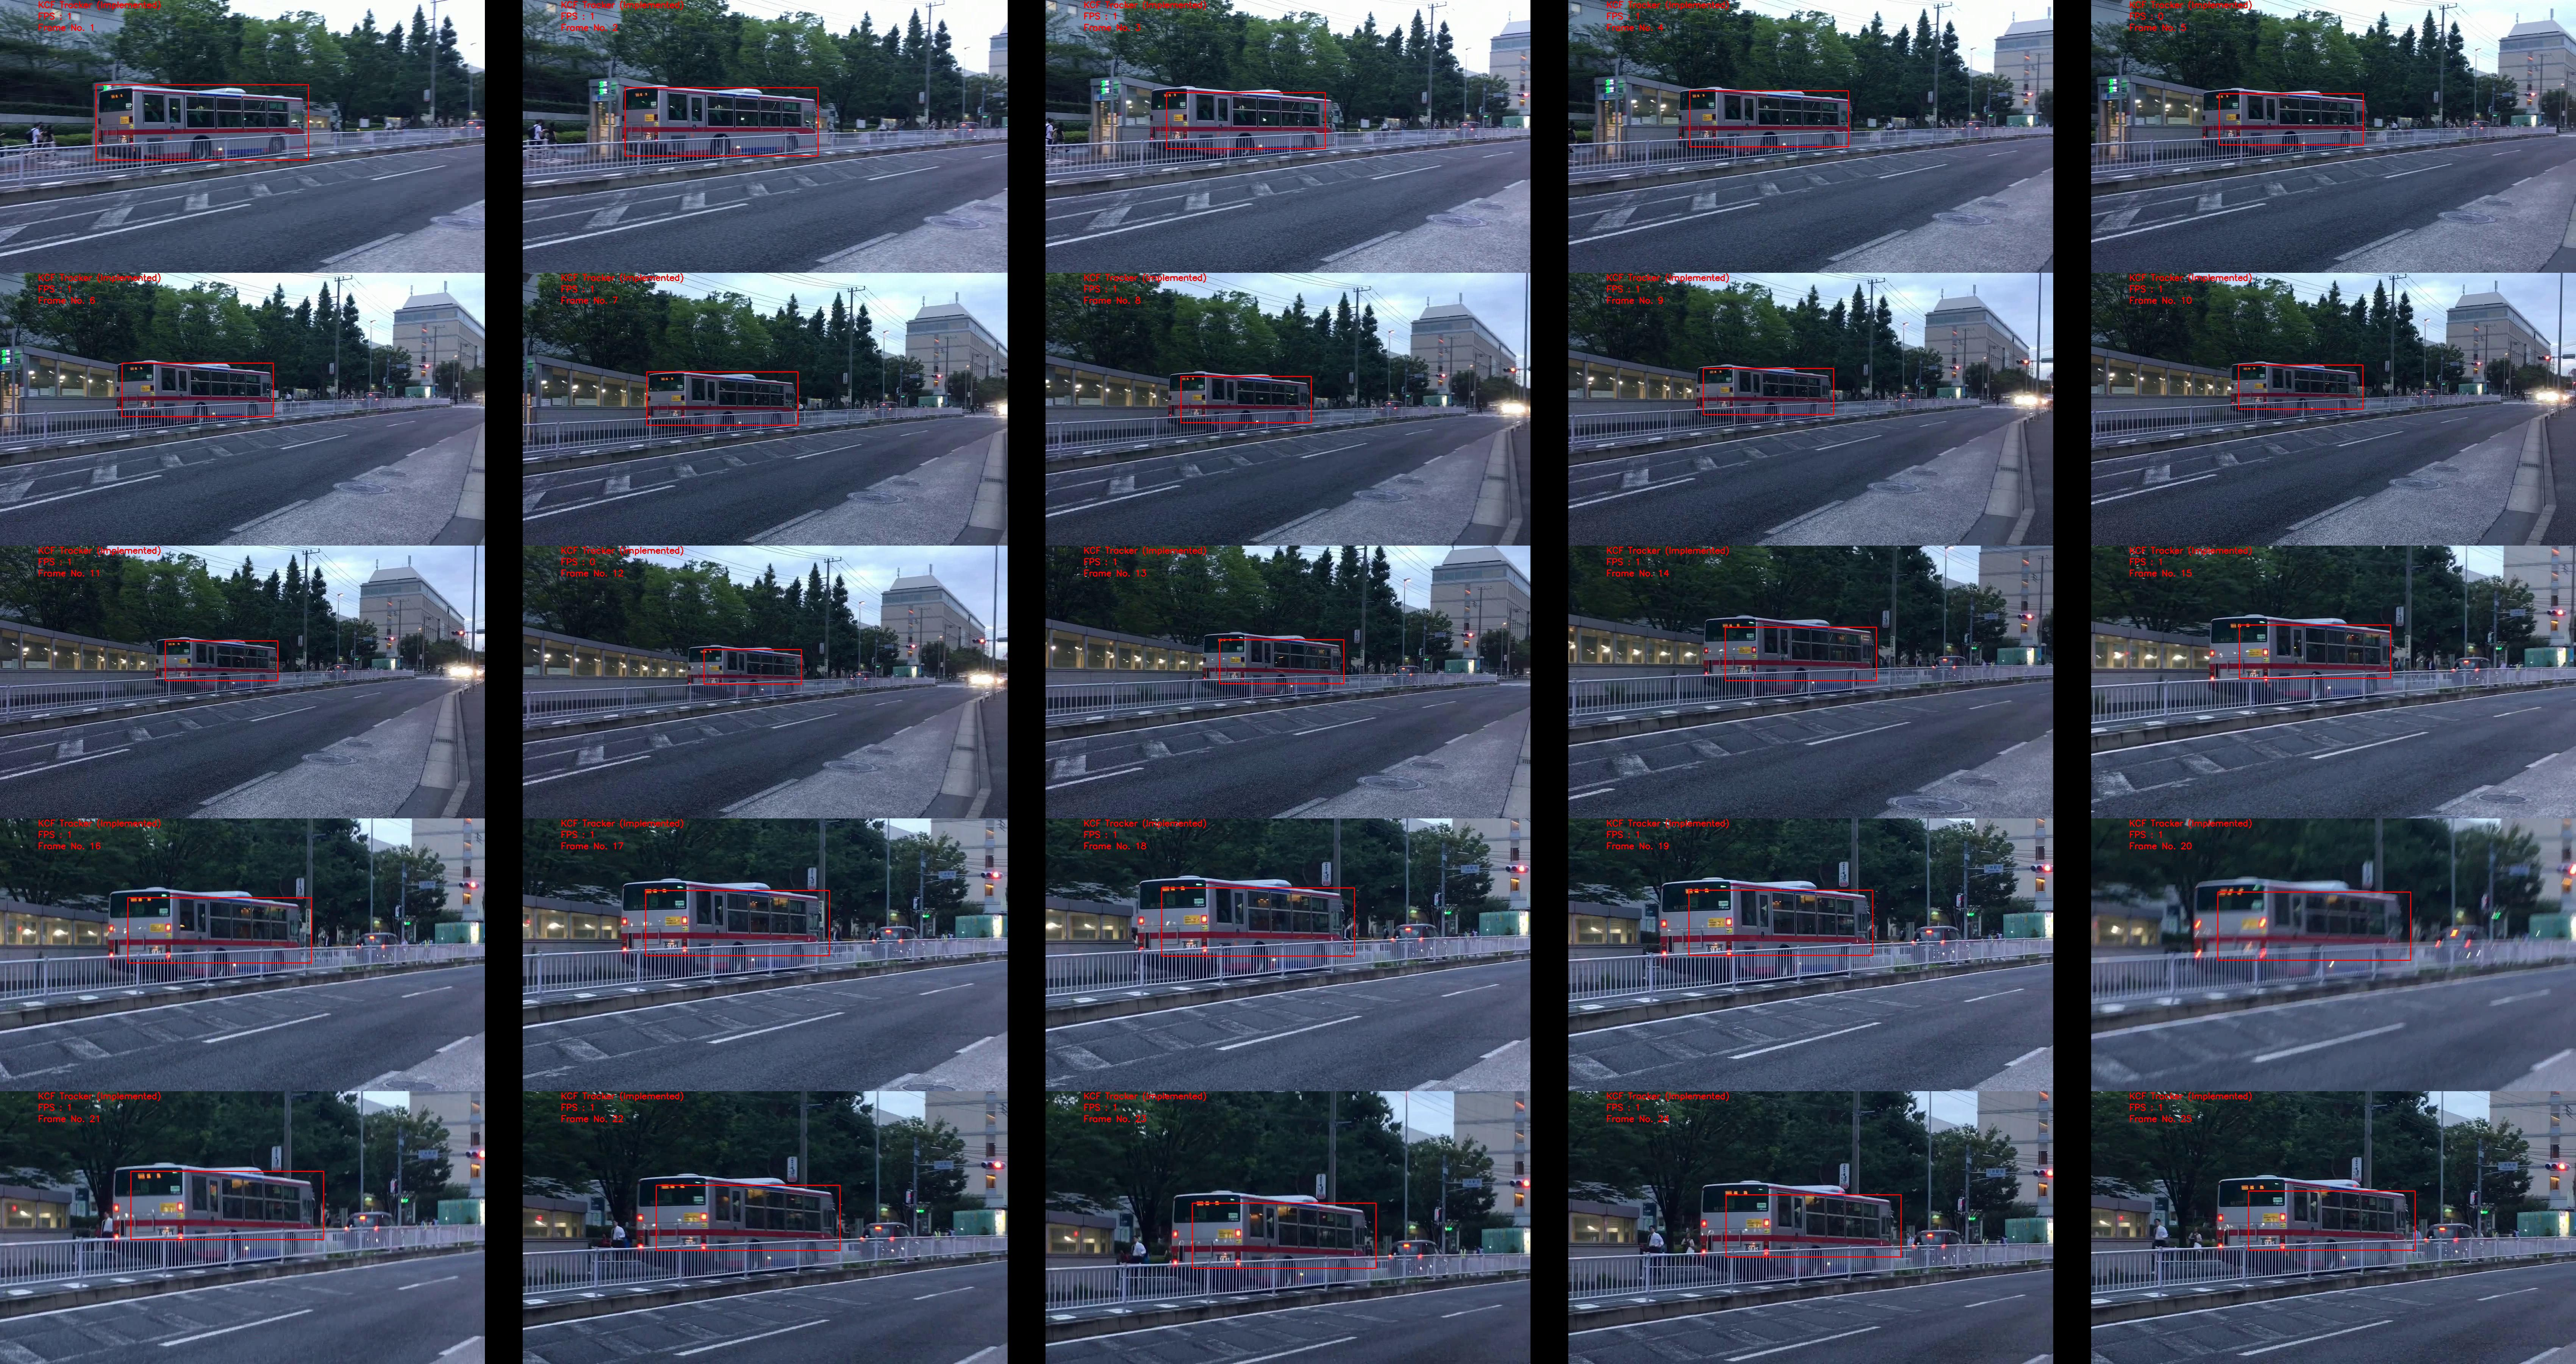
\includegraphics[clip,width=12.5cm]{./figures/bus1_kcf_impl.jpg}
        \caption{bus1.mp4に対して,実装した KCF Trackerで物体追跡を行なった結果}
        \label{fig:AC_PetriNet}
      \end{center}
    \end{figure}

  \section{考察}
  
  \section{結論}

    \begin{itemize}
      \item foo
      \item bar
      \item buz
    \end{itemize}

  \bibliography{ref} % ref.bibから拡張子を外した名前
  \bibliographystyle{junsrt} % 参考文献出力スタイル
\end{document}
